\documentclass[stu, 12pt, letterpaper, donotrepeattitle, floatsintext, natbib]{apa7}
\usepackage[utf8]{inputenc}
%\usepackage{fontspec} %paquete para usar la fuente Arial 12
\usepackage{comment}
\usepackage{marvosym}
\usepackage{graphicx}
\usepackage{float}
\usepackage[normalem]{ulem}
\usepackage[spanish]{babel} 
\usepackage{lastpage} %para le formato que quiere la profe QUITAR SI QUIERES OG APA7
\usepackage{ragged2e} %para le formato que quiere la profe QUITAR SI QUIERES OG APA7
\usepackage{indentfirst} %para le formato que quiere la profe QUITAR SI QUIERES OG APA7

\setcounter{secnumdepth}{0} %permite enumerar las secciones QUITAR SI QUIERES OG APA7

%comando para ajustar la fuente Arial en todo el documento
%\setmainfont{Arial} %COMPILAR DOC CON XeLateX DOS VECES

\DeclareCaptionLabelSeparator*{spaced}{\\[2ex]}
\captionsetup[table]{textfont=it,format=plain,justification=justified,
  singlelinecheck=false,labelsep=spaced,skip=1pt}

\selectlanguage{spanish}

\useunder{\uline}{\ul}{}
\newcommand{\myparagraph}[1]{\paragraph{#1}\mbox{}\\}

%\rfoot{Página \thepage \hspace{1pt} de \pageref{LastPage}}%QUITAR SI QUIERES OG APA7 
\rhead{} %QUITAR SI QUIERES OG APA7
\setcounter{secnumdepth}{3} %permite enumerar las secciones QUITAR SI QUIERES OG APA7
\setlength{\parindent}{1.27cm} %sangria forzada QUITAR SI QUIERES OG APA7

\renewcommand\labelitemi{$\bullet$}

\newcommand*\chem[1]{\ensuremath{\mathrm{#1}}}

\begin{document}
    %PORTADA
    \begin{titlepage}
        \begin{figure}[ht]
            \centering
            
\includegraphics[width=15cm]{logosITT.png}
        \end{figure}
        \centering
        {\Large Tecnológico Nacional de México\\Instituto Tecnológico de Tijuana\par}
        \vspace{1cm}
        {\Large SCD-1011SC6C Ingeniería de Software\par}
        \vspace{1cm}
        {\Large Unidad 1\par}
        \vspace{2cm}
        {\Large\bfseries Tarea 2\par}
        \vspace{2cm}
        {\large Dra. Martha Elena Pulido\par}
        \vfill
            {\large Abraham Jhared Flores Azcona, 19211640\par}
        \vfill
        {\large 15 de febrero de 2021}
    \end{titlepage}

% Índices
\pagenumbering{arabic}
    % Contenido
\renewcommand\contentsname{Contenido}
\tableofcontents

% Cuerpo 
    %NOTA: PARA CITAR ESTILO "Merts (2003)" usar \cite{<nombre_cita_bib>}
    %                        "(Metz, 1978)" usar \citep{<nombre_cita_bib>}
\newpage
\section{Introducción}
Las \begin{justifying}
    necesidades que se espera cumplír con un proyecto requieren de una serie de guías para poder realizarse sin muchos inconvenientes. En esta breve redacción se explican las cinco
    metodologías más populares en la industria para poder crear otras más equiparadas o seguir las establecidas para futura referencia.\par
    \end{justifying}
\vspace{\baselineskip}    
\section{Procesos de Software}
\subsection{Definición}
A \begin{justifying}
    grandes rasgos, los procesos de software son los conjuntos de actividades y resultados asociados que producen el producto de software.
    Dichas actividades pueden envolver el desarrollo de software desde cero o la modificación de un sistema existente. \citep{geeksforgeeks-2021, elgabry-2022,unknown-author-no-dateA}\par
  \end{justifying}
\vspace{\baselineskip}
\subsection{Ejemplos}
Debido \begin{justifying}
    a que existen distintos objetivos que se puedan logra con el desarrollo de dicho proyecto, existen distintas metodologías que pueden aplicarse, pero las más populares son las siguientes: \citep{vats-2022} \emph{de cascada, iterativo, incremental, espiral, ágil, etc.}.
    Cabe destacar que partiendo de estos modelos, se pueden concebír otros que acomoden de manera más específica distintas necesidades.\par
\end{justifying}
\subsubsection{De cascada}
Representa \begin{justifying}
    el desensamble de las actividades del proyecto de software en una fase secuencial lineal. Cada fase se remonta en las partes derivables de la fase anterior, y esto corresponde a los aspectos
    particulares de los deberes. Cada etapa del modelo es completada antes de la siguiente fase para evitar traspasarse hacia otras fases.\par
\end{justifying}
\begin{figure}[H]
    \caption{\emph{Diagrama del modelo de cascada\\}}
    \centering
    \smallskip
    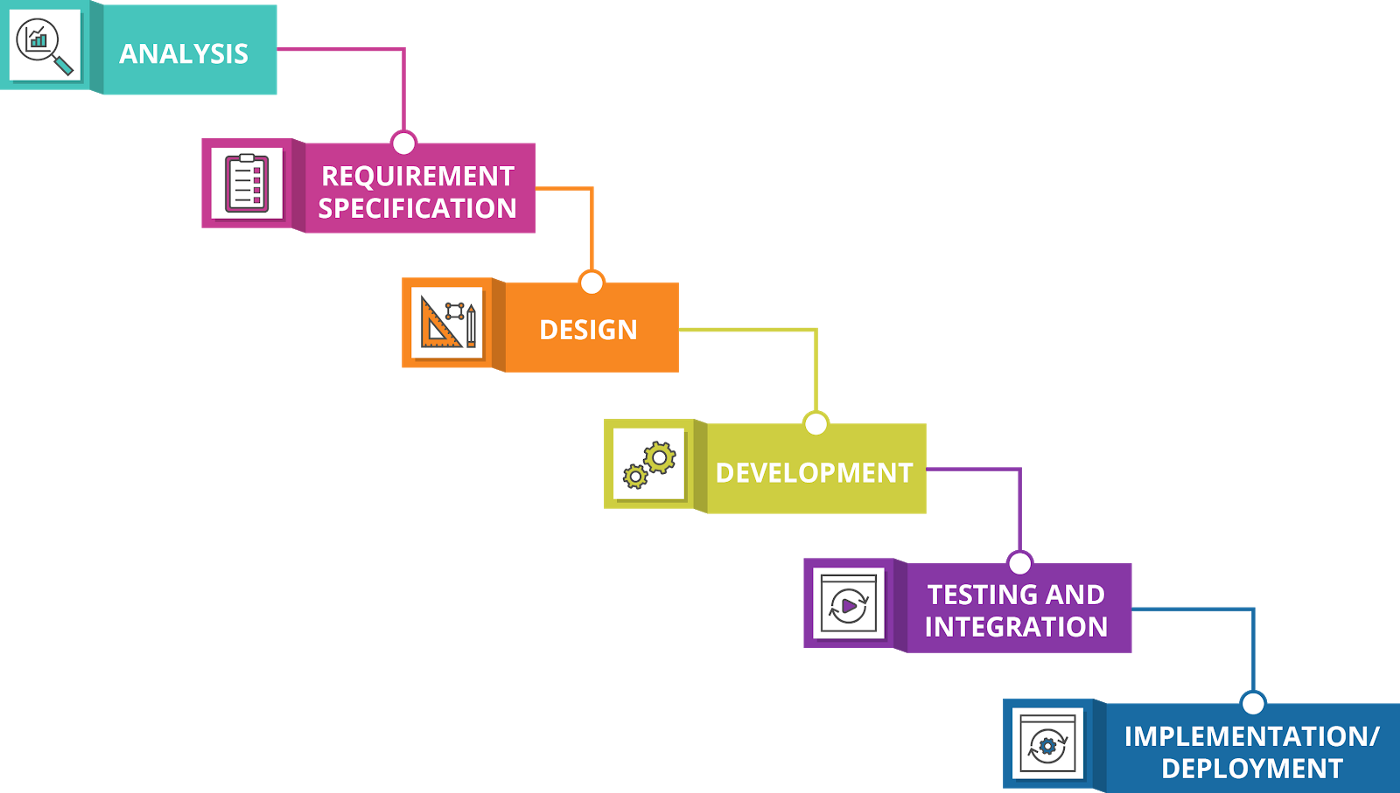
\includegraphics[width=12cm, height=8cm]{waterfall.png}
    \bigskip
    \justifying\small\textit{Nota}. Tomado de \cite{waddell-2021}.%citar al de medium del waterfall
\end{figure}
\vspace{\baselineskip}
\subsubsection{Iterativo}
Comparado \begin{justifying}
    al resto de modelos, éste empieza enfocandoze en un conjunto simplificado e inicial de las actividades y características. Dichas características se desarrollan
    progresivamente para ganar complejidad y un gran rango de funciones hasta que el sistema esperado está terminado.\par
\end{justifying}
\begin{figure}[H]
    \caption{\emph{Diagrama del modelo iterativo\\}}
    \centering
    \smallskip
    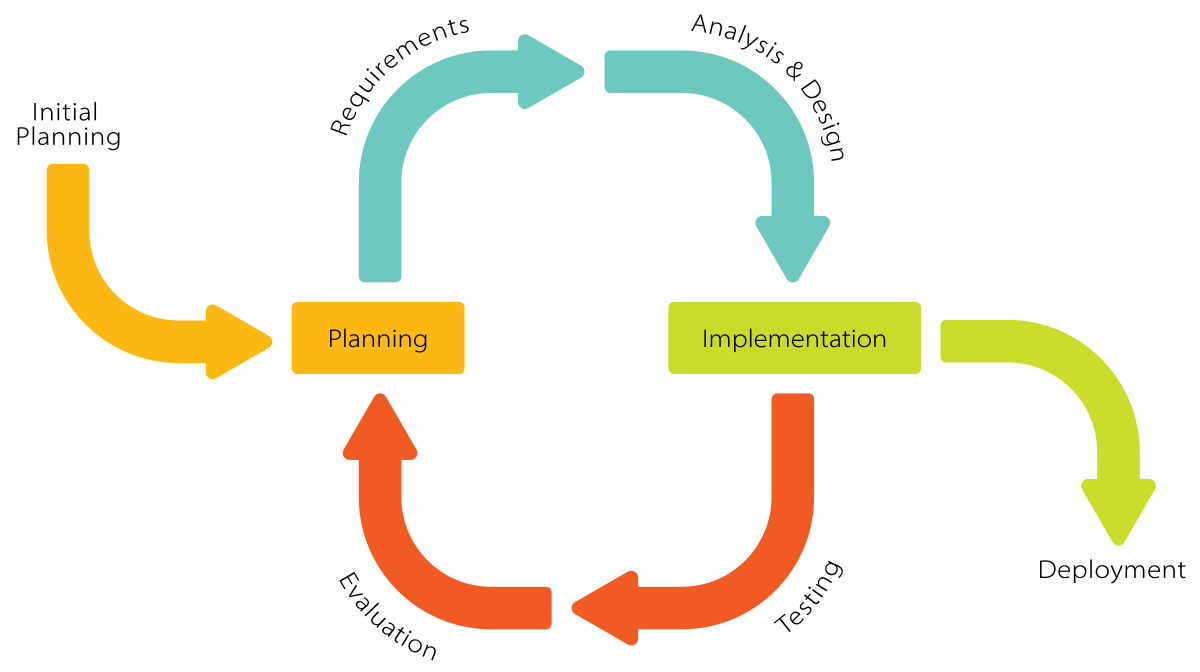
\includegraphics[width=12cm, height=8cm]{iterative.png}
    \bigskip
    \justifying\small\textit{Nota}. Tomado de \cite{wikipedia-contributors-2021}. %citar a wikipedia
\end{figure}
\vspace{\baselineskip}
\subsubsection{Incremental}
Es \begin{justifying}
    un modelo en el cual el programa es diseñado, implementado y probado cuidadosamente hasta que el proyecto se obtiene. Dico proceso envuelve tanto a los aspectos de desarrollo como
los de mantenimiento.\par
\end{justifying}
\begin{figure}[H]
    \caption{\emph{Diagrama del modelo incremental\\}}
    \centering
    \smallskip
    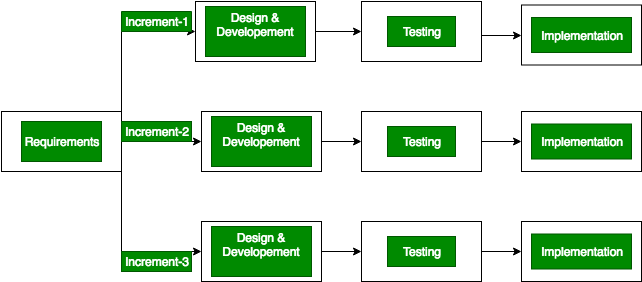
\includegraphics[width=12cm, height=8cm]{incremental.png}
    \bigskip
    \justifying\small\textit{Nota}. Tomado de \cite{geeksforgeeks-2019}%citar a geeks for geeks
\end{figure}
\vspace{\baselineskip}
\subsubsection{Espiral}
Se \begin{justifying}
    al modelo enfocado en el desarrollo de software con pruebas. Cada espiral se conoce como la fase del proceso entero de desarrollo. Las fases totales requeridas para desarrollar el software
    pueden diferir de administradores de proyectos y dependen de los riesgos asociados.\par
\end{justifying}
\begin{figure}[H]
    \caption{\emph{Diagrama del modelo espiral\\}}
    \centering
    \smallskip
    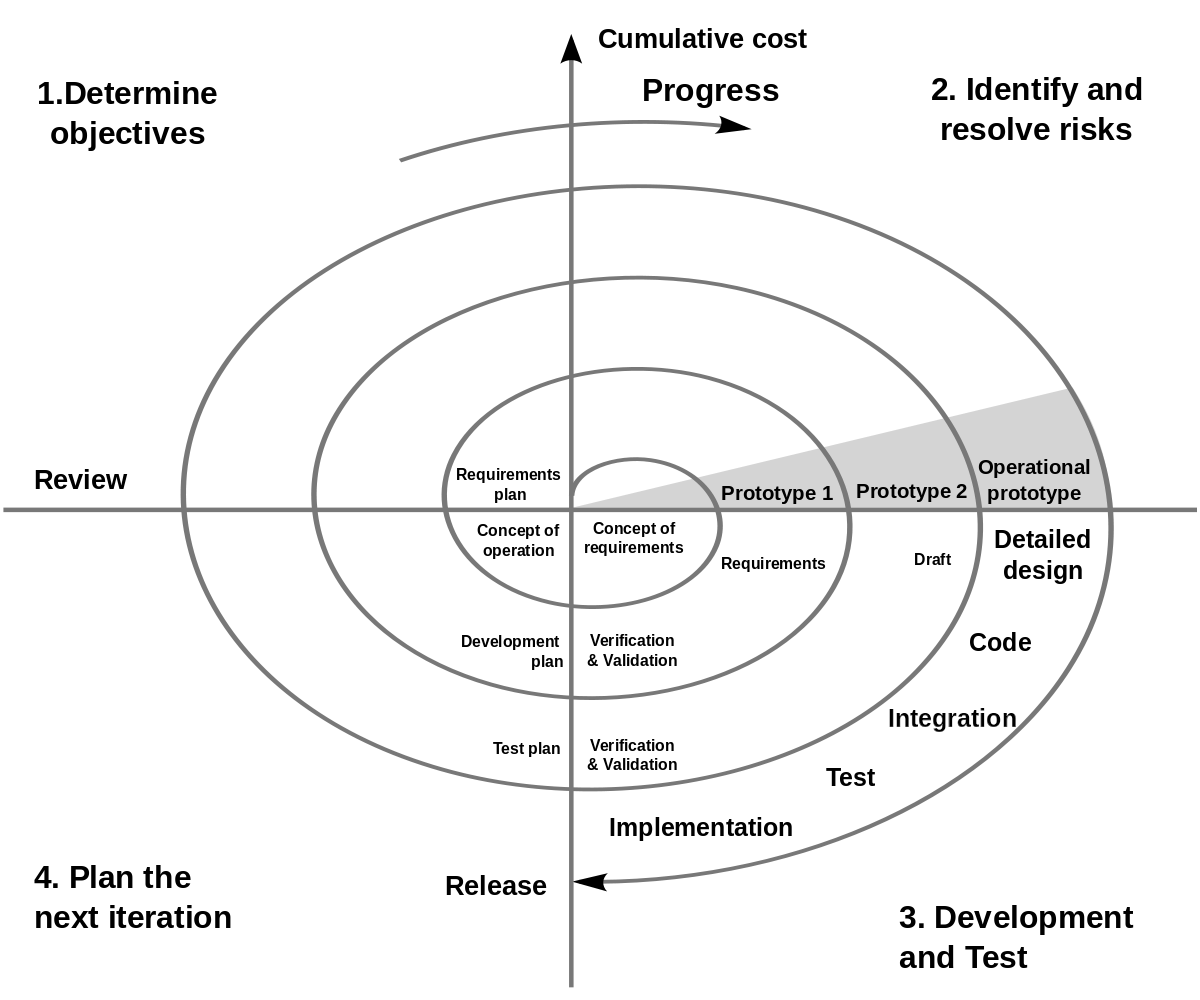
\includegraphics[width=12cm, height=8cm]{spiral.png}
    \bigskip
    \justifying\small\textit{Nota}. Tomado de \cite{wikipedia-contributors-2022}%citar a wikipedia
\end{figure}
\vspace{\baselineskip}
\subsubsection{Agil}
Es \begin{justifying}
    un término coloquial que refiere a un conjunto específico de prácticas y métodos basados en los valores de dicha metodología. Dichos valores representan una manera de pensar que
    permite a los negocios y miembros del equipo a inovar rápidamente y a responder a las demandas siempre cambiantes de la industria mientras se eliminan los riesgos. Marcos de trabajo comunes que
    soportan dicha metodología son Kanban, Lean, Scrum, etc.\par
\end{justifying}
\begin{figure}[H]
    \caption{\emph{Diagrama del modelo ágil\\}}
    \centering
    \smallskip
    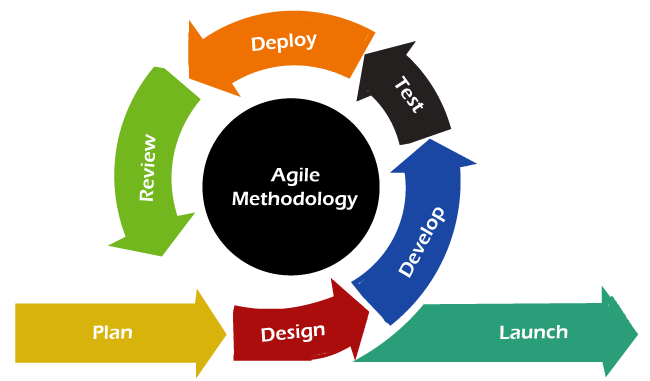
\includegraphics[width=12cm, height=8cm]{agile.png}
    \bigskip
    \justifying\small\textit{Nota}. Tomado de \cite{unknown-author-no-dateB}.%citar a wikipedia
\end{figure}
\vspace{\baselineskip}
\section{Conclusión}
Como \begin{justifying}
    se aprecia, los tipos de modelos ofrecen distintos enfoques que permiten alcanzar el objetivo final de los proyectos donde se aplicasen.\par
\end{justifying}
\renewcommand\refname{\textbf{Referencias}}
\bibliography{referencias} %el archivo 'referencias.bib' debe estar dentro del mismo folder donde se encuentra el archivo .tex para citar las referencias deseadas

\end{document}